\documentclass{article}
\usepackage[utf8]{inputenc}
\usepackage[T1]{fontenc}
\usepackage[toc,page]{appendix}
\usepackage{xcolor}
\usepackage{amsmath,amssymb,bm,cancel,xspace}
\usepackage{graphicx}
\usepackage[colorlinks=true,allcolors=blue]{hyperref}
\usepackage[left=1in,right=1in,bottom=1in,top=1in]{geometry}
\usepackage[backend=biber,sorting=none]{biblatex}
\addbibresource{notes.bib}

\newcommand{\igm}{\textsc{IllinoisGRMHD}\xspace}
\newcommand{\zl}{\textsc{ZelmaniLeak}\xspace}
\newcommand{\cactus}{\textsc{Cactus}\xspace}
\newcommand{\etk}{\textsc{Einstein Toolkit}\xspace}
\newcommand{\stellarcollapse}{\texttt{stellarcollapse.org}\xspace}

\newcommand{\prd}{Physical Review D}
\newcommand{\apj}{Americal Physics Journal}

\newcommand{\primv}{\bm{P}}
\newcommand{\consv}{\bm{C}}
\newcommand{\fluxv}{\bm{F}}
\newcommand{\sourcev}{\bm{S}}
\newcommand{\mhd}{{\rm MHD}}
\newcommand{\ye}{Y_{\rm e}}
\newcommand{\yet}{\tilde{Y}_{\rm e}}
\newcommand{\sqrtgamma}{\sqrt{\gamma}}
\newcommand{\etal}{\textit{et al.}\xspace}
\newcommand{\dF}{{^{^*}\!\!F}}
\newcommand{\What}{\hat{W}}
\newcommand{\BdotS}{B\cdot S}
\newcommand{\Sdotn}{S\cdot n}
\newcommand{\bdotn}{b\cdot n}
\newcommand{\udotB}{u\cdot B}
\newcommand{\vdotB}{\varv\cdot B}
\newcommand{\ent}{\mathcal{S}}
\newcommand{\entstar}{\tilde{\ent}}
\newcommand{\Eps}{\mathcal{E}}
\renewcommand{\ne}{n_{\rm e}}
\newcommand{\nb}{n_{\rm b}}
\newcommand{\mb}{m_{\rm b}}
\newcommand{\siegel}{\cite{siegel2018recovery}\xspace}
\newcommand{\palenzuela}{\cite{palenzuela2015effects}\xspace}
\newcommand{\todo}[1]{{\color{red}\bf TO DO: #1}\xspace}
\newcommand{\Ptot}{P_{\rm tot}}

\DeclareSymbolFont{matha}{OML}{txmi}{m}{it}% txfonts
\DeclareMathSymbol{\varv}{\mathord}{matha}{118}

\newcommand{\eq}[1]{
\begin{equation}
    #1
\end{equation}
}

\newcommand{\eqnn}[1]{
\begin{equation*}
    #1
\end{equation*}
}

\newcommand{\spl}[1]{
\eq{
\begin{split}
    #1
\end{split}
}
}

\newcommand{\splnn}[1]{
\eqnn{
\begin{split}
    #1
\end{split}
}
}

\newcommand{\al}[1] {
\begin{align}
    #1
\end{align}
}

\title{Notes on \igm}
\author{Leonardo Werneck}
\date{November 2020}


\begin{document}

\maketitle

\tableofcontents

\section{Introduction}

These are notes that will summarize the changes made to \igm so that it can work with tabulated equations of state (EOS), particularly the open-source tables of Schneider, Roberts, and Ott (SRO)~\cite{schneider2017open}, and the open-source, \cactus/\etk neutrino leakage thorn \zl~\cite{2012PhRvD..86b4026O,2013ApJ...768..115O}, both of which are available at \stellarcollapse.

We will give an overview of the general relativistic magnetohydrodynamics (GRMHD) formalism and the difference and similarities between the variables used by each code. We will also discuss in detail the equations used by the new conservative-to-primitive (C2P) inversion scheme that is adopted by \igm, due to Palenzuela \etal~\palenzuela. Finally, we will go into detail about the modifications required to implement the neutrino leakage scheme in \igm.

\section{GRMHD equations (no leakage)}

In units where $G = c = M_{\odot} = 1$, Einstein's equations become

\eq{ G^{\mu\nu} = 8\pi T^{\mu\nu}\ ,\label{eq:EinsteinsEqs} }

\noindent where $G^{\mu\nu}$ is the Einstein tensor and $T^{\mu\nu}$ is the total energy-momentum tensor. The GRMHD equations are given by:

\al{
\nabla_{\mu}\left(\nb u^{\mu}\right) &= 0\ ,\label{eq:ConsBaryonNumber}\\
\nabla_{\mu}\left(\ne u^{\mu}\right) &= 0\ ,\label{eq:ConsLeptonNumber}\\
\nabla_{\mu}\left(\ent u^{\mu}\right)   &= 0\ ,\label{eq:ConsEntropy}\\
\nabla_{\mu}T^{\mu\nu} &= 0\ ,\label{eq:ConsEM}\\
\nabla_{\nu}\dF^{\mu\nu} &= 0\ ,\label{eq:MaxwellsEqs}
}

\noindent which are, respectively, the baryon number conservation equation, the lepton number conservation equation, the entropy conservation equation, the energy-momentum conservation equations, and Maxwell's equations. In the equations above, $\nabla_{\mu}$ is the covariant derivative compatible with the spacetime metric $g_{\mu\nu}$, $\nb (\ne)$ is the  number density of baryons (leptons), $u^{\mu}$ is the fluid 4-velocity, $\ent$ is the entropy, $F^{\mu\nu}$ is the Faraday tensor, with $\dF^{\mu\nu} = (1/2)\epsilon^{\mu\nu\rho\sigma}F_{\rho\sigma}$ its dual, and $\epsilon^{\mu\nu\rho\sigma}$ is the Levi-Civita tensor.

We note the new equations~\eqref{eq:ConsLeptonNumber} and~\eqref{eq:ConsEntropy}, which are added to the standard set of GRMHD equations. The purpose of the two will be made clear soon.

The conservation of baryon number equation is usually replaced by

\spl{
0 &= \nabla_{\mu}\left(n_{b}u^{\mu}\right)\\
  &= \frac{m_{b}}{m_{b}}\nabla_{\mu}\left(n_{b}u^{\mu}\right)\\
  &= \frac{1}{m_{b}}\nabla_{\mu}\left(m_{b}n_{b}u^{\mu}\right)\\
  &= \nabla_{\mu}\left(\rho u^{\mu}\right)\ ,
}

\noindent where $\rho = n_{b}m_{b}$ is the fluid rest-mass density. Similarly, the conservation of lepton number equation is usually replaced by

\spl{
0 &= \mb\nabla_{\mu}\left(\ne u^{\mu}\right)\\
  &= \nabla_{\mu}\left(\mb\ne u^{\mu}\right)\\
  &= \nabla_{\mu}\left[\left(\nb\mb\right)\left(\frac{\ne}{\nb}\right) u^{\mu}\right]\\
  &= \nabla_{\mu}\left(\rho\ye u^{\mu}\right)\ ,
}

\noindent where $\ye \equiv \ne/\nb$ is the \emph{electron fraction}.

In order to solve equations~\eqref{eq:EinsteinsEqs}--\eqref{eq:MaxwellsEqs} numerically, we use the standard 3+1 ADM decomposition of the metric $g_{\mu\nu}$

\eq{
ds^{2} = \left(-\alpha^{2}+\beta^{\ell}\beta_{\ell}\right)dt^{2}
       + 2\beta_{i}\,dt\, dx^{i}
       + \gamma_{ij}\,dx^{i}\,dx^{j}\ ,
}

\noindent where $\alpha$ is the lapse function, $\beta^{i}$ is the shift vector, and $\gamma_{ij}$ is the ADM 3-metric. Spacetime evolution is performed using the BSSN formalism.

To evolve the GRMHD quantities, the GRMHD equations are rewritten in \emph{conservative form} in the ideal MHD limit ($u_{\mu}F^{\mu\nu}=0$),

\eq{ \partial_{t}\consv + \nabla_{i}\fluxv^{i} = \sourcev\ , \label{eq:ConservEvol}}

\noindent where $\consv$ is the vector of \emph{conservative} variables, $\fluxv^{i}$ is the flux vector along direction $i$, and $\sourcev$ is the vector of source terms. The vectors $\consv$, $\fluxv^{i}$, and $\sourcev$ depend directly on the so-called \emph{primitive} variables $\primv$. All of these vectors are typically implementation dependent, and we will discuss the ones of interest over the next sections.

\section{Conservative-to-primitive}

\igm defines the set of \emph{primitive} variables

\eq{
\primv = 
\begin{bmatrix}
\rho\\
P\\
v^{i}\\
B^{i}\\
\ye\\
\ent
\end{bmatrix}\ ,
}

\noindent where $P$ is the pressure, $v^{i} \equiv u^{i}/u^{0}$ is the fluid 3-velocity, with $u^{\mu}$ is the fluid 4-velocity, and $B^{i}$ are the spatial components of the magnetic field ($B^{\mu}$) measured by normal (or Eulerian) observers with 4-velocity $n^{\mu} = \left(\alpha^{-1},-\alpha^{-1}\beta^{i}\right)$ and is normal to the spatial hypersurface, $B^{\mu}n_{\mu}=0$, as well as the metric and its derivatives. Note that the electron fraction $\ye$ and the entropy $\ent$ are added to the list of original primitive variables presented in~\cite{etienne2015illinoisgrmhd}.

The \emph{conserved} variables, which are the ones evolved in time using the method of lines (MoL) and equation~\eqref{eq:ConservEvol}, are given by

\eq{
\consv = 
\begin{bmatrix}
\tilde{D}\\
\tilde{\tau}\\
\tilde{S}_{i}\\
\tilde{B}^{i}\\
\yet\\
\entstar
\end{bmatrix}
\equiv
\sqrtgamma
\begin{bmatrix}
D\\
\tau\\
S_{i}\\
B^{i}\\
D\ye\\
W \ent
\end{bmatrix}
\equiv
\sqrtgamma
\begin{bmatrix}
W\rho\\
n_{\mu}n_{\nu}T^{\mu\nu} - D\\
-n_{\mu}T^{\mu}_{\ i}\\
B^{i}\\
D\ye\\
W \ent
\end{bmatrix}
=
\sqrtgamma
\begin{bmatrix}
W\rho\\
\alpha^{2}T^{00} - D\\
\alpha T^{0}_{\ i}\\
B^{i}\\
D\ye\\
W \ent
\end{bmatrix}\ ,
}

\noindent where $\gamma=\det\left(\gamma_{ij}\right)$, $\gamma_{ij}$ is the ADM 3-metric, $W=\alpha u^{0} = \left(1-\gamma_{ij}v^{i}v^{j}\right)^{-1/2}$ is the Lorentz factor, and $n_{\mu}=\left(-\alpha,0,0,0\right)$. The GRMHD energy-momentum tensor, $T^{\mu\nu}$, is given by

\eq{
T^{\mu\nu} = \left(\rho h + b^{2}\right)u^{\mu}u^{\nu} + \left(P + P_{\rm mag}\right) g^{\mu\nu} - b^{\mu}b^{\nu}\ ,
}

\noindent where $h = 1 + \epsilon + P/\rho$ is the specific enthalpy, $\epsilon$ the specific internal energy, $P_{\rm mag} = b^{2}/2$, $b^{2} \equiv g_{\mu\nu}b^{\mu}b^{\nu}$, $b^{\mu} \equiv B^{\mu}_{(u)}/\sqrt{4\pi}$, and

\al{
B^{0}_{(u)} &= \frac{u_{i}B^{i}}{\alpha}\ ,\label{eq:B0u}\\
B^{i}_{(u)} &= \frac{B^{i}/\alpha + B^{0}_{(u)}u^{i}}{u^{0}}\label{eq:Biu}\ .
}

There are no analytic formulas that would allow us to recover the primitive variables $\primv$ directly from the conserved variables $\consv$. Recovering the primitive variables is a crucial step in any GRMHD code, and special routines are designed to handle this task. These routines require a root-finding algorithm, of which the most popular (and robust) one is the Newton-Raphson method, but other methods are also used (as we will see later).

Even in simplest models which allow us to fully specify the fluid by, say, the primitives $\left(\rho,P,v^{x},v^{y},v^{z}\right)$, we still must  recover 5 primitive variables\footnote{The recovery of the magnetic fields is trivial since the conserved and primitive magnetic fields are both the same quantity.}. Naively one would assume that this would involve solving a system of 5 non-linear equations, and although this can certainly be done, the resulting inversion scheme is not the most robust one~\cite{noble2006primitive}. Using identities obtained from the conserved variables allow us to reduce the number of equations used, and robust algorithms can be developed to solve these equations, resulting in less recovery failures. In the following sections we will discuss all the routines available in \igm.

\subsection{The Noble \etal recovery schemes}

The standard conservative-to-primitive routine in \igm is due to Noble \etal~\cite{noble2006primitive}. The routine solves two non-linear equations using a Newton-Raphson root-finder, and is thus referred to as a ``2D'' recovery scheme. Alternatively, one can further reduce the number of equations to one, yielding a ``1D'' recovery scheme. We now present a full derivation of the equations used by such schemes.

We start by introducing the 4-dimensional version of the conserved variable $S_{i}$, namely

\spl{
S_{\mu} &= -n_{\nu}T^{\nu}_{\ \mu}\\
        &= \alpha T^{0}_{\ \mu}\\
        &= \alpha\left[\left(\rho h+b^{2}\right)u^{0}u_{\mu} + \left(P+P_{\rm mag}\right)\delta^{0}_{\ \mu} - b^{0}b_{\mu}\right]\\
        &= W\left(\rho h + b^{2}\right)u_{\mu} -\Ptot n_{\mu} + \left(b^{\nu}n_{\nu}\right)b_{\mu}\ ,\label{eq:Smu1}
}

\noindent where we have used $\Ptot \equiv P + P_{\rm mag}$, $W=\alpha u^{0}$, $n_{\mu} = \left(-\alpha,0,0,0\right)=-\alpha\delta^{0}_{\ \mu}$, and $\alpha b^{0} = -b^{\mu}n_{\mu}=-\bdotn$. For the derivations that follow, it is useful to introduce the variable

\eq{
z \equiv \rho h W^{2}\ ,
}

\noindent and rewrite equations \eqref{eq:B0u} and \eqref{eq:Biu} in the more compact form\footnote{Note that while we are missing a factor of $\left(4\pi\right)^{-1/2}$ in these equations, they become simpler and easier to understand than if we keep carrying the factors of $\left(4\pi\right)^{-1/2}$ throughout the derivations. Note that this trick is also used in the code: prior the conservative-to-primitive function call, we rescale the magnetic fields by $\left(4\pi\right)^{-1/2}$.}

\eq{
b^{\mu} = \frac{B^{\mu} + \left(\udotB\right)u^{\mu}}{W}\ .
}

\noindent Remembering that $u^{\mu}u_{\mu}=-1$, we find that

\spl{
b^{2} &\equiv b^{\mu}b_{\mu}\\
      &= \left[\frac{B^{\mu} + \left(\udotB\right)u^{\mu}}{W}\right]
         \left[\frac{B_{\mu} + \left(\udotB\right)u_{\mu}}{W}\right]\\
      &= \frac{B^{\mu}B_{\mu} + \left(\udotB\right)^{2}u^{\mu}u_{\mu} + 2\left(\udotB\right)^{2}}{W^{2}}\\
\implies b^{2}&= \frac{1}{W^{2}}\left[B^{2} + \left(\udotB\right)^{2}\right]\ .
}

\noindent Another useful identity is

\eq{
\bdotn = \frac{\cancelto{0}{n_{\mu}B^{\mu}} + \left(\udotB\right)n_{\mu}u^{\mu}}{W} = -\udotB\ .
}

\noindent In terms of $z$ and the magnetic field $B^{\mu}$, we can rewrite equation~\eqref{eq:Smu1} as

\spl{
S_{\mu} &= W\rho h u_{\mu} + W b^{2} u_{\mu} - \Ptot n_{\mu} + \left(\Sdotn\right)b_{\mu}\\
&= \frac{z}{W}u_{\mu} + \left[\frac{B^{2}+\left(\udotB\right)^{2}}{W}\right]u_{\mu} - \Ptot n_{\mu} - \left(\udotB\right)\left[\frac{B_{\mu} + \left(\udotB\right)u_{\mu}}{W}\right]\\
&= \frac{z}{W}u_{\mu} + \frac{B^{2}}{W}u_{\mu} + \cancel{\frac{\left(\udotB\right)^{2}}{W}u_{\mu}} - \Ptot n_{\mu} - \frac{\left(\udotB\right)}{W}B_{\mu} -\cancel{\frac{\left(\udotB\right)^{2}}{W}u_{\mu}}\\
& = \left(\frac{z+B^{2}}{W}\right)u_{\mu} - \Ptot n_{\mu} - \frac{\left(\udotB\right)}{W}B_{\mu}\ .\label{eq:Smu2}
}

\noindent From this last equation we find the key result

\spl{
\BdotS &\equiv B^{\mu}S_{\mu}\\
       &= \left(\frac{z + \cancel{B^{2}}}{W}\right)\left(\udotB\right) - \cancelto{0}{\Ptot n_{\mu}B^{\mu}} - \cancel{\frac{\left(\udotB\right)}{W}B^{2}}\\
      &= \frac{z}{W}\left(\udotB\right)\\
\implies \udotB &= \frac{W}{z}\left(\BdotS\right)\ .\label{eq:udotB}
}

\noindent Using~\eqref{eq:udotB} in \eqref{eq:Smu2} we find

\eq{
S_{\mu} = \left(\frac{z+B^{2}}{W}\right)u_{\mu} - \Ptot n_{\mu} - \frac{\left(\BdotS\right)}{z}B_{\mu}\ .\label{eq:Smufinal}
}

\noindent At this point we then define

\eq{
\hat{S}_{\mu} \equiv S_{\mu} + \left(\Sdotn\right)n_{\mu}\ ,
}

\noindent where

\spl{
\Sdotn &= -z-B^{2} + \Ptot\ ,\label{eq:Sdotn}
}

\noindent yielding

\spl{
\hat{S}_{\mu} &= \left(\frac{z+B^{2}}{W}\right)u_{\mu} - \cancel{\Ptot n_{\mu}} - \frac{\left(\BdotS\right)}{z}B_{\mu} - \left(z+B^{2}\right)n_{\mu} + \cancel{\Ptot n_{\mu}}\\
&= \left(\frac{z+B^{2}}{W}\right)u_{\mu} - \left(z+B^{2}\right)n_{\mu} - \frac{\left(\BdotS\right)}{z}B_{\mu}\ .\label{eq:Shatmufinal}
}

Our goal is now to compute $\hat{S}^{2} \equiv \hat{S}^{\mu}\hat{S}_{\mu}$. In order to do so, we will need a few other identities. Let us start from $\hat{S}^{\mu}u_{\mu}$:

\spl{
    \hat{S}^{\mu}u_{\mu} &= u^{\mu}\hat{S}_{\mu}\\
    &=-\left(\frac{z+B^{2}}{W}\right) +W\left(z+B^{2}\right)-\frac{\left(\BdotS\right)}{z}\left(\udotB\right)\\
    &= \left(z+B^{2}\right)\left(W-\frac{1}{W}\right) - \frac{W}{z^{2}}\left(\BdotS\right)^{2}\ .
}

\noindent Then we note that

\eq{
\hat{S}^{\mu}n_{\mu} = S^{\mu}n_{\mu} + \left(\Sdotn\right)n^{\mu}n_{\mu} = 0\ .
}

\noindent Finally, we compute $\hat{S}^{\mu}B_{\mu}$:

\eq{
\hat{S}^{\mu}B_{\mu} = S^{\mu}B_{\mu} + \left(\Sdotn\right)n^{\mu}B_{\mu} = \BdotS\ .
}

Using all these identities we compute

\spl{
\hat{S}^{2} &= \left(\frac{z+B^{2}}{W}\right)\left(\hat{S}^{\mu}u_{\mu}\right) - \left(z+B^{2}\right)\cancelto{0}{\left(\hat{S}^{\mu}n_{\mu}\right)} - \frac{\left(\BdotS\right)}{z}\left(\hat{S}^{\mu}B_{\mu}\right)\\
&=\left(\frac{z+B^{2}}{W}\right)\left[\left(z+B^{2}\right)\left(W-\frac{1}{W}\right) - \frac{W}{z^{2}}\left(\BdotS\right)^{2}\right] - \frac{\left(\BdotS\right)^{2}}{z}\\
&=\left(z+B^{2}\right)\underbrace{\left(1 - \frac{1}{W^{2}}\right)}_{v^{2}} - \frac{\left(z+B^{2}\right)\left(\BdotS\right)^{2}}{z^{2}} - \frac{\left(\BdotS\right)^{2}}{z}\ ,
}

\noindent which leads to equation (27) in~\cite{noble2006primitive}

\eq{
\boxed{\hat{S}^{2} = \left(z+B^{2}\right)v^{2} - \frac{\left(2z+B^{2}\right)\left(\BdotS\right)}{z^{2}}}\ ,\label{eq:Noble_Shatsquared}
}

\noindent Solving this for $v^{2}$ then yields equation (28) in~\cite{noble2006primitive}

\eq{
\boxed{v^{2} = \frac{z^{2}\hat{S}^{2} + \left(2z+B^{2}\right)\left(\BdotS\right)^{2}}{z^{2}\left(z+B^{2}\right)^{2}}}\ .\label{eq:Noble_vsq}
}

The other equation we use comes from the contraction~\eqref{eq:Sdotn},

\spl{
  n^{\mu}S_{\mu} &= -z+B^{2}+\Ptot\\
  &= -z + B^{2} + P + \frac{b^{2}}{2}\\
  &= -z + B^{2} + P + \frac{1}{2W^{2}}\left[B^{2} + \left(\udotB\right)^{2}\right]\\
  &= -z + B^{2} + P + \frac{B^{2}}{2W^{2}} + \frac{1}{2W^{2}}\left[\frac{W^{2}}{z^{2}}\left(\BdotS\right)^{2}\right]\\
  &= \frac{B^{2}}{2}\underbrace{\left(\frac{1}{W^{2}}-2\right)}_{-(1+v^{2})} + \frac{\left(\BdotS\right)^{2}}{2z^{2}} - z + P\ ,
}

\noindent yielding equation (29) in~\cite{noble2006primitive}

\eq{
\boxed{ \Sdotn = -\frac{B^{2}}{2}\left(1+v^{2}\right) + \frac{\left(\BdotS\right)^{2}}{2z^{2}} - z + P }\ .\label{eq:Noble_z}
}

There are 4 different schemes supported by \igm which are based on the set of equations we have just found. The first one solves equations~\eqref{eq:Noble_vsq} and~\eqref{eq:Noble_z} on the variables $z$ and $v^{2}$ using a 2D Newton-Raphson routine. The second scheme substitutes $v^{2}$ in equation~\eqref{eq:Noble_z} using~\eqref{eq:Noble_vsq}, yielding a single equation on the variable $z$, which is then solved using a 1D Newton-Raphson routine. A third scheme uses equation~\eqref{eq:Noble_Shatsquared} and the entropy, which is recovered analytically using $\entstar = \ent/W$. Finally, a fourth scheme also adopts the entropy and a slightly modified version of equation~\eqref{eq:Noble_Shatsquared}, which is obtained in the following way. First, recall that $D = W \rho$. Then, one can compute

\eq{
  v^{2} = 1 - \frac{1}{W^{2}} = 1 - \frac{\rho^{2}}{D^{2}} = \frac{D^{2}-\rho^{2}}{D^{2}} = \frac{\left(D+\rho\right)\left(D-\rho\right)}{D^{2}}\ .
}

\noindent Using this last result in equation~\eqref{eq:Noble_Shatsquared}, and multiplying the result by $z^{2}$ yields

\eq{
  \boxed{\frac{1}{D^{2}}\left\{z^{2}\left[D^{2}\tilde{S}^{2} - \left(D-\rho\right)\left(D+\rho\right)\left(B^{2}+z\right)^{2} + D^{2}\left(\BdotS\right)^{2}\left(B^{2}+2W\right)\right]\right\} = 0}\ .
}

Once the Newton-Raphson method has converged, we will have $z$ and $v^{2}$. Note that for the 1D routines this is still true, since $v^{2}$ can be directly computed from $z$ and the conserved variables using equation~\eqref{eq:Noble_vsq}. At this point, $W$ can be computed from $v^{2}$ and thus $\rho = D/W$ can also be determined. The pressure can be recovered using the equation of state, while the velocities can be recovered using equation~\eqref{eq:Smufinal}. We have

\eq{
  S^{\mu} = \left(\frac{z+B^{2}}{W}\right)u^{\mu} - \left(z+B^{2}\right)n^{\mu} - \frac{\left(\BdotS\right)}{z}B^{i}\ ,
}

\noindent which we can then recast as

\eq{
  u^{\mu} - Wn^{\mu}= \left(\frac{W}{z+B^{2}}\right)\left[S^{\mu}+\frac{\left(\BdotS\right)}{z}B^{i}\right]\ .
}

\noindent Picking the spatial components and defining the velocity $\tilde{u}^{i} \equiv u^{i} + W\beta^{i}/\alpha$, we have

\eq{
\boxed{\tilde{u}^{i} = \left(\frac{W}{z+B^{2}}\right)\left[S^{i}+\frac{\left(\BdotS\right)}{z}B^{i}\right]}\ .\label{eq:C2P_velocities}
}

\noindent The velocities used by the \igm code, $v^{i} = u^{i}/u^{0}$, can then be recovered using

\eq{
  v^{i} = \frac{\tilde{u}^{i}}{u^{0}} - \beta^{i}\ .
}

\subsection{The Palenzuela \etal scheme}

The Palenzuela \etal recovery scheme~\cite{neilsen2014magnetized} (see also~\cite{siegel2018recovery} for an excellent review) has been successfully used for binary neutron star simulations which adopt realistic nuclear equations of state. Because of this, it is the default routine in \igm when such equations of state are used. Such equations of state require us to evolve the electron fraction and keep track of the temperature throughout the evolution. The recovery of the electron fraction is, however, analytic, using $\ye = D\ye/D$. We note that this scheme is somewhat ideal for \igm, because it only requires guess for the temperature, and furthermore the guess need not be perfect. Since \igm does not keep track of the primitive variables in between time steps, it relies heavily on routines that can be robust even with poor initial guesses, and that is the case for the Palenzuela \etal scheme.

Before proceeding, it is instructuve to pause and set the notation we will be using below. While in the discussion of the previous section we were very careful in defining 4-vectors, such as $\hat{S}_{\mu}$, for which the raising operation $\hat{S}^{\mu} = g^{\mu\nu}\hat{S}_{\nu}$ is clearly well-defined, and thus $\hat{S}^{2} \equiv \hat{S}^{\mu}\hat{S}_{\mu}$ is a reasonable notation to use, we often find in the literature the definition (see e.g.~\cite{neilsen2014magnetized,siegel2018recovery,giacomazzo2007whiskymhd,cerda2008new,anton2006numerical})

\eq{
S^{2} \equiv S^{i}S_{i} = \gamma^{ij}S_{i}S_{j}\ .
}

\noindent If we define the velocity

\eq{
  \varv^{i} \equiv \frac{\gamma^{i}_{\ \mu}u^{\mu}}{-n_{\mu}u^{\mu}}\quad ,\quad \varv_{i} \equiv \frac{\gamma_{i\mu}u^{\mu}}{-n_{\mu}u^{\mu}}\ ,
}

\noindent where $\gamma_{\mu\nu} = g_{\mu\nu} + n_{\mu}n_{\nu}$ is the induced metric, we find

\eq{
  \varv^{i} = \frac{u^{i} - Wn^{i}}{W} = \frac{u^{i}}{W} + \frac{\beta^{i}}{\alpha} = \frac{\tilde{u}^{i}}{W}\ ,
}

\noindent and

\eq{
  \varv_{i} = \frac{u_{i} - Wn_{i}}{W} = \frac{u_{i}}{W} = \frac{\tilde{u}_{i}}{W}\ .\label{eq:varvD}
}

\noindent Using this velocity and identity~\eqref{eq:udotB}, we find

\eq{
  \vdotB = \varv_{i}B^{i} = \frac{u_{i}}{W}B^{i} = \frac{1}{W}\left[\frac{W}{z}\left(\BdotS\right)\right] = \frac{\left(\BdotS\right)}{z}\ .
}

\noindent Picking the spatial components of relation~\eqref{eq:Smufinal} and using~\eqref{eq:varvD} we get

\eq{
  S_{i} = \left(z + B^{2}\right)\varv_{i} - \frac{\left(\BdotS\right)}{z}B_{i}\ ,
}

\noindent and finally, using $B^{2} = B^{\mu}B_{\mu} = B^{i}B_{i} = \gamma^{ij}B_{i}B_{j}$ and $v^{2} = \gamma^{ij}\varv_{i}\varv_{j}$, we find

\spl{
  S^{2} &\equiv \gamma^{ij}S_{i}S_{j}\\
  &= \gamma^{ij}\left[\left(z + B^{2}\right)\varv_{i} - \frac{\left(\BdotS\right)}{z}B_{i}\right]\left[\left(z + B^{2}\right)\varv_{j} - \frac{\left(\BdotS\right)}{z}B_{j}\right]\\
  &= \left(z+B^{2}\right)v^{2} -2\frac{\left(z+B^{2}\right)\left(\BdotS\right)}{z}\left(\vdotB\right) + \frac{\left(\BdotS\right)^{2}}{z^{2}}B^{2}\\
  &= \left(z+B^{2}\right)v^{2} -\frac{\left(2z+\cancel{2}B^{2}\right)\left(\BdotS\right)^{2}}{z^{2}} + \cancel{\frac{\left(\BdotS\right)^{2}}{z^{2}}B^{2}}\\
  &= \left(z+B^{2}\right)v^{2} - \frac{\left(2z+B^{2}\right)\left(\BdotS\right)^{2}}{z^{2}}\\
  &= \hat{S}^{2}\ .
}

\noindent This last result allows us to drop the hat notation and use $S^{2}$ throughout the discussion that follows.

We now describe the scheme in detail. Having gone through the derivation of the equations used by the Noble \etal schemes, we already have everything we need at our disposal. Following Palenzuela \etal~\cite{neilsen2014magnetized} we define

\eq{
q \equiv \frac{\tau}{D}\ \ ,\
r \equiv \frac{S^{2}}{D^{2}}\ \ ,\
s \equiv \frac{B^{2}}{D}\ \ ,\
t \equiv \frac{\BdotS}{D^{3/2}}\ ,\label{eq:qrst}
}

\noindent and the auxiliary variable

\eq{
x \equiv \frac{z}{D} = h W\ ,\label{eq:Palenzuela_x}
}

\noindent which is bounded by~\siegel (\todo{why?})

\eq{ 1+q-s < x < 2 + 2q - s \ .}

Using equation~\eqref{eq:Noble_vsq} and the definitions of $r$, $s$, $t$, and $x$, we have

\spl{
  v^{2} &= 1 - W^{-2}\\
  &= \frac{\left(D^{2}x^{2}\right)\left(D^{2}r\right) + \left[2\left(Dx\right) + \left(Ds\right)\right]\left[D^{3}t^{2}\right]}{D^{2}x^{2}\left[Dx + Ds\right]^{2}}\\
  &= \frac{\cancel{D^{4}}}{\cancel{D^{4}}}\left[\frac{x^{2}r + \left(2x+s\right)t^{2}}{x^{2}\left(x+s\right)^{2}}\right]\ ,
}

\noindent or, rearranging a bit,

\eq{
  \boxed{ W^{-2} = 1 - \frac{x^{2}r + \left(2x+s\right)t^{2}}{x^{2}\left(x+s\right)^{2}} }\ .\label{eq:Palenzuela_Wminus2}
}

To get to the second key result, we start from the definition of the conserved energy $\tau$,

\spl{
  \tau &= n_{\mu}n_{\nu}T^{\mu\nu} - D\\
  &= \alpha^{2}T^{00} - D\\
  &= \alpha^{2}\left[\left(\rho h + b^{2}\right)\left(u^{0}\right)^{2} + \left(P + \frac{b^{2}}{2}\right)g^{00} - \left(b^{0}\right)^{2}\right] - D\\
  &=\left(\rho h + b^{2}\right)W^{2} - P - \frac{b^{2}}{2} - \left(\udotB\right)^{2} - D\ ,\label{eq:tau1}
}
  
\noindent where in the last equality we have used the identity $\alpha b^{0} = -\bdotn = \udotB = D^{1/2} W t / x$. Noting that $\rho h =  W^{-2} D x$, we can find an expression for the pressure

\spl{
  P &= \left[\frac{D x + B^{2} + \cancel{\left(\udotB\right)^{2}}}{\bcancel{W^{2}}}\right]\bcancel{W^{2}} - \frac{B^{2}}{2W^{2}} - \frac{\left(\udotB\right)^{2}}{2W^{2}} - \cancel{\left(\udotB\right)^{2}} - D - \tau\\
  &= D x + D s - \frac{D s}{2W^{2}} - \frac{1}{2\cancel{W^{2}}}\left(\frac{\cancel{W^{2}} t^{2} D}{x^{2}}\right) - D - D q\\
  &= \rho W\left[x + s - \frac{1}{2}\left(\frac{s}{W^{2}} + \frac{t^{2}}{x^{2}}\right) - 1 - q\right]\ .
}

\noindent Then from the expression for the enthalpy we can find the specific internal energy:

\spl{
  \epsilon &= h - 1 - \frac{P}{\rho}\\
  &= - 1 + \frac{x}{W} - W\left[x + s - \frac{1}{2}\left(\frac{s}{W^{2}} + \frac{t^{2}}{x^{2}}\right) - 1 - q\right]\\
  &= - 1 + \frac{x}{W} - xW + W\left[1 + q - s + \frac{1}{2}\left(\frac{s}{W^{2}} + \frac{t^{2}}{x^{2}}\right)\right]\ ,
}

\noindent finally resulting in

\eq{
  \boxed{ \epsilon = - 1 + \frac{x}{W}\left(1 - W^{2}\right) + W\left[1 + q - s + \frac{1}{2}\left(\frac{s}{W^{2}} + \frac{t^{2}}{x^{2}}\right)\right] }\ .\label{eq:Palenzuela_eps}
}

The Palenzuela \etal scheme then uses Brent's method in order to find $x$ such that

\eq{ f(x) \equiv x - h W = 0 \ .}

\noindent Starting from the bounds $x_{\rm low} = 1+q-s$ and $x_{\rm high} = 2+2q-s$, we perform the following iterative procedure (hatted quantities are computed at each iteration):

\begin{enumerate}
\item Using equation~\eqref{eq:Palenzuela_Wminus2}, compute $\hat{W}$.
\item Compute $\hat{\rho} = D/\hat{W}$.
\item Using equation~\eqref{eq:Palenzuela_eps}, compute $\hat{\epsilon}$.
\item Using the EOS, compute $\hat{T}=T\left(\hat{\rho},\ye,\hat{\epsilon}\right)$ and then $\hat{P}=P\left(\hat{\rho},\ye,\hat{T}\right)$.
\item Use Brent's method to solve for $x$ using $f(x) = x - \hat{h}\hat{W} = x - \left(1 + \hat{\epsilon} + \hat{P}/\hat{\rho}\right)\hat{W}$.
\end{enumerate}

Steps 1-5 above are repeated iteratively until $f(x)$ has converged to a user specified tolerance. After convergence, $W$ is computed using equation~\eqref{eq:Palenzuela_Wminus2}, $\rho = D/W$, $\epsilon$ is given by equation~\eqref{eq:Palenzuela_eps}, $P$ and $T$ are computed using the EOS, and the velocities are obtained using equation~\eqref{eq:C2P_velocities}.

We have introduced a modification of this routine in \igm which is important to discuss here. Whenever we are in a region of table parameters in which $d\epsilon/dT \ll 1$, step 4 above can become incredibly innacurate when determining the temperature $T$. This usually does not spoil the GRMHD evolution since other quantities, such as the pressure, will also have a very weak temperature dependence. However, since this issue usually affects high density, low temperature regions, it is difficult to evolve cold neutron star initial data in such a way that the star remains cold throughout the evolution. To remedy this issue, we have introduced a threshold parameter, $\delta$, and whenever $d\epsilon/dT < \delta$ we replace steps 3 and 4 above with the following steps:

\begin{enumerate}
\setcounter{enumi}{3}
\item Compute the entropy $\hat{\ent} = \left(W\ent\right) / \hat{W}$.
\item Using the EOS, compute $\hat{T} = T\left(\hat{\rho},\ye,\hat{\ent}\right)$, $\hat{P}=P\left(\hat{\rho},\ye,\hat{T}\right)$, and $\hat{\epsilon}=\epsilon\left(\hat{\rho},\ye,\hat{T}\right)$.
\end{enumerate}

\noindent It is also relevant to mention that using the entropy equation leads to a less robust algorithm, particularly in the atmospheric regions close to the surface of neutron stars. Because of this, even when the criterion $d\epsilon/dT < \delta$ is satisfied, if the recovery fails when using the entropy we perform a new recovery attempt using the standard scheme.

\subsection{The Newman \& Hamlin scheme}

Starting from~\eqref{eq:tau1} we have

\spl{
  \tau + D + P &= \left(\rho h + b^{2}\right)W^{2} - \frac{b^{2}}{2} - \left(\udotB\right)^{2}\\
  &= \rho h W^{2} + B^{2} + \cancel{\left(\udotB\right)^{2}} - \frac{B^{2}}{2W^{2}} - \frac{\left(\udotB\right)^{2}}{2W^{2}} - \cancel{\left(\udotB\right)^{2}}\\
  &= \left(z + B^{2}\right) - \frac{B^{2}}{2W^{2}} - \frac{\left(\BdotS\right)^{2}}{2z^{2}}\ .
}

\noindent Defining the total energy $e \equiv \tau + D$ and adding $B^{2}/2$ to both sides of the last equation we get

\spl{
  e + P + \frac{B^{2}}{2} &= \left(z + B^{2}\right) \frac{B^{2}}{2}\left( 1 - \frac{1}{1W^{2}}\right) - \frac{\left(\BdotS\right)^{2}}{2z^{2}}\\
  &= \left(z + B^{2}\right) + \frac{B^{2}v^{2}}{2} - \frac{\left(\BdotS\right)^{2}}{2z^{2}}\\
  &= \left(z + B^{2}\right) + \frac{1}{2}\left[B^{2}v^{2} - \frac{\left(\BdotS\right)^{2}}{z^{2}}\right]\ .\label{eq:Newman1}
}

\noindent We now seek an identity for the terms inside the square braces. We start from equation~\eqref{eq:Noble_vsq} multiplied by $B^{2}$:

\eq{
  B^{2}v^{2} = \frac{S^{2}B^{2}}{\left(z+B^{2}\right)^{2}} + \frac{B^{2}\left(2z + B^{2}\right)\left(\BdotS\right)^{2}}{z^{2}\left(z+B^{2}\right)^{2}}\ .
}

\noindent Now subtract $\left(\BdotS\right)^{2}/z^{2}$ from both sides, to get the desired combination:

\spl{
  B^{2}v^{2} - \frac{\left(\BdotS\right)^{2}}{z^{2}} &= \frac{S^{2}B^{2}}{\left(z+B^{2}\right)^{2}} + \frac{B^{2}\left(2z + B^{2}\right)\left(\BdotS\right)^{2}}{z^{2}\left(z+B^{2}\right)^{2}} - \frac{\left(\BdotS\right)^{2}}{z^{2}}\\
  &= \frac{S^{2}B^{2}}{\left(z+B^{2}\right)^{2}} + \frac{B^{2}\left(2z+B^{2}\right)\left(\BdotS\right)^{2} - \left(z+B^{2}\right)^{2}\left(\BdotS\right)^{2}}{z^{2}\left(z+B^{2}\right)^{2}}\\
  &= \frac{S^{2}B^{2}}{\left(z+B^{2}\right)^{2}} + \frac{\left(\BdotS\right)^{2}}{z^{2}\left(z+B^{2}\right)^{2}}\left(\cancel{2zB^{2}} + \bcancel{B^{4}} - z^{2} - \bcancel{B^{4}} - \cancel{2zB^{2}}\right)\\
  &= \frac{S^{2}B^{2} - \left(\BdotS\right)^{2}}{\left(z+B^{2}\right)^{2}}\ .\label{eq:Newman2}
}

\noindent Substituting~\eqref{eq:Newman2} into~\eqref{eq:Newman1} we find

\eq{
  e + P + \frac{B^{2}}{2} = \left(z+B^{2}\right) + \frac{1}{2}\left[\frac{B^{2}S^{2} - \left(\BdotS\right)^{2}}{\left(z+B^{2}\right)^{2}}\right]\ .\label{eq:Newman3}
}

\noindent Defining the auxiliary variables

\al{
  \Eps &\equiv z + B^{2}\ ,\\
  a &\equiv e + P + \frac{B^{2}}{2}\ ,\\
  d &\equiv \frac{B^{2}S^{2} - \left(\BdotS\right)^{2}}{2}\ ,
}

\noindent we can write~\eqref{eq:Newman3} as the cubic equation

\eq{
  \boxed{\Eps^{3} - a\Eps^{2} + d = 0}\ .
}

\noindent From their definitions, it also follows that $a>0$ and $d\geq0$. Defining the polynomial

\eq{
  f\left(\Eps\right) = \Eps^{3} - a\Eps^{2} + d\ ,\label{eq:Newmanf}
}

\noindent we find the extrema

\eq{
  0 = \frac{df\left(\Eps\right)}{d\Eps} = 3\Eps^{2} - 2a\Eps \implies \Eps = \left\{
    \begin{matrix}
      0\\
      2a/3
    \end{matrix}
    \right.
}

\noindent Because $\Eps > 0$, we focus exclusively on the extremum $2a/3$. Analysing the second derivative of $f(\Eps)$ at this point we find

\eq{
  \left.\frac{d^{2}f}{d\Eps^{2}}\right|_{\Eps=2a/3} = \left.\left[6\Eps - 2a\right]\right|_{\Eps=2a/3} = 2a > 0\ .
}

\noindent Therefore, the inflection point $\Eps=2a/3$ will cause the derivative of $f(\Eps)$ to change signs, from negative to positive. It follows, therefore, that a positive-valued root of $f(\Eps)$ can only be found if $f(2a/3)\leq0$, which imposes a constraint on $d$:

\eq{
  f\left(2a/3\right) = \frac{8a^{3}}{27} - \frac{4a}{9} + d = - \frac{4a^{3}}{27} + d \leq 0 \implies d \leq \frac{4a^{3}}{27}\ .
}

\noindent We provide a visual representation of the argument that lead to this last result in figure~\ref{fig:f_of_Eps}.

\begin{figure}[!htb]
    \centering
    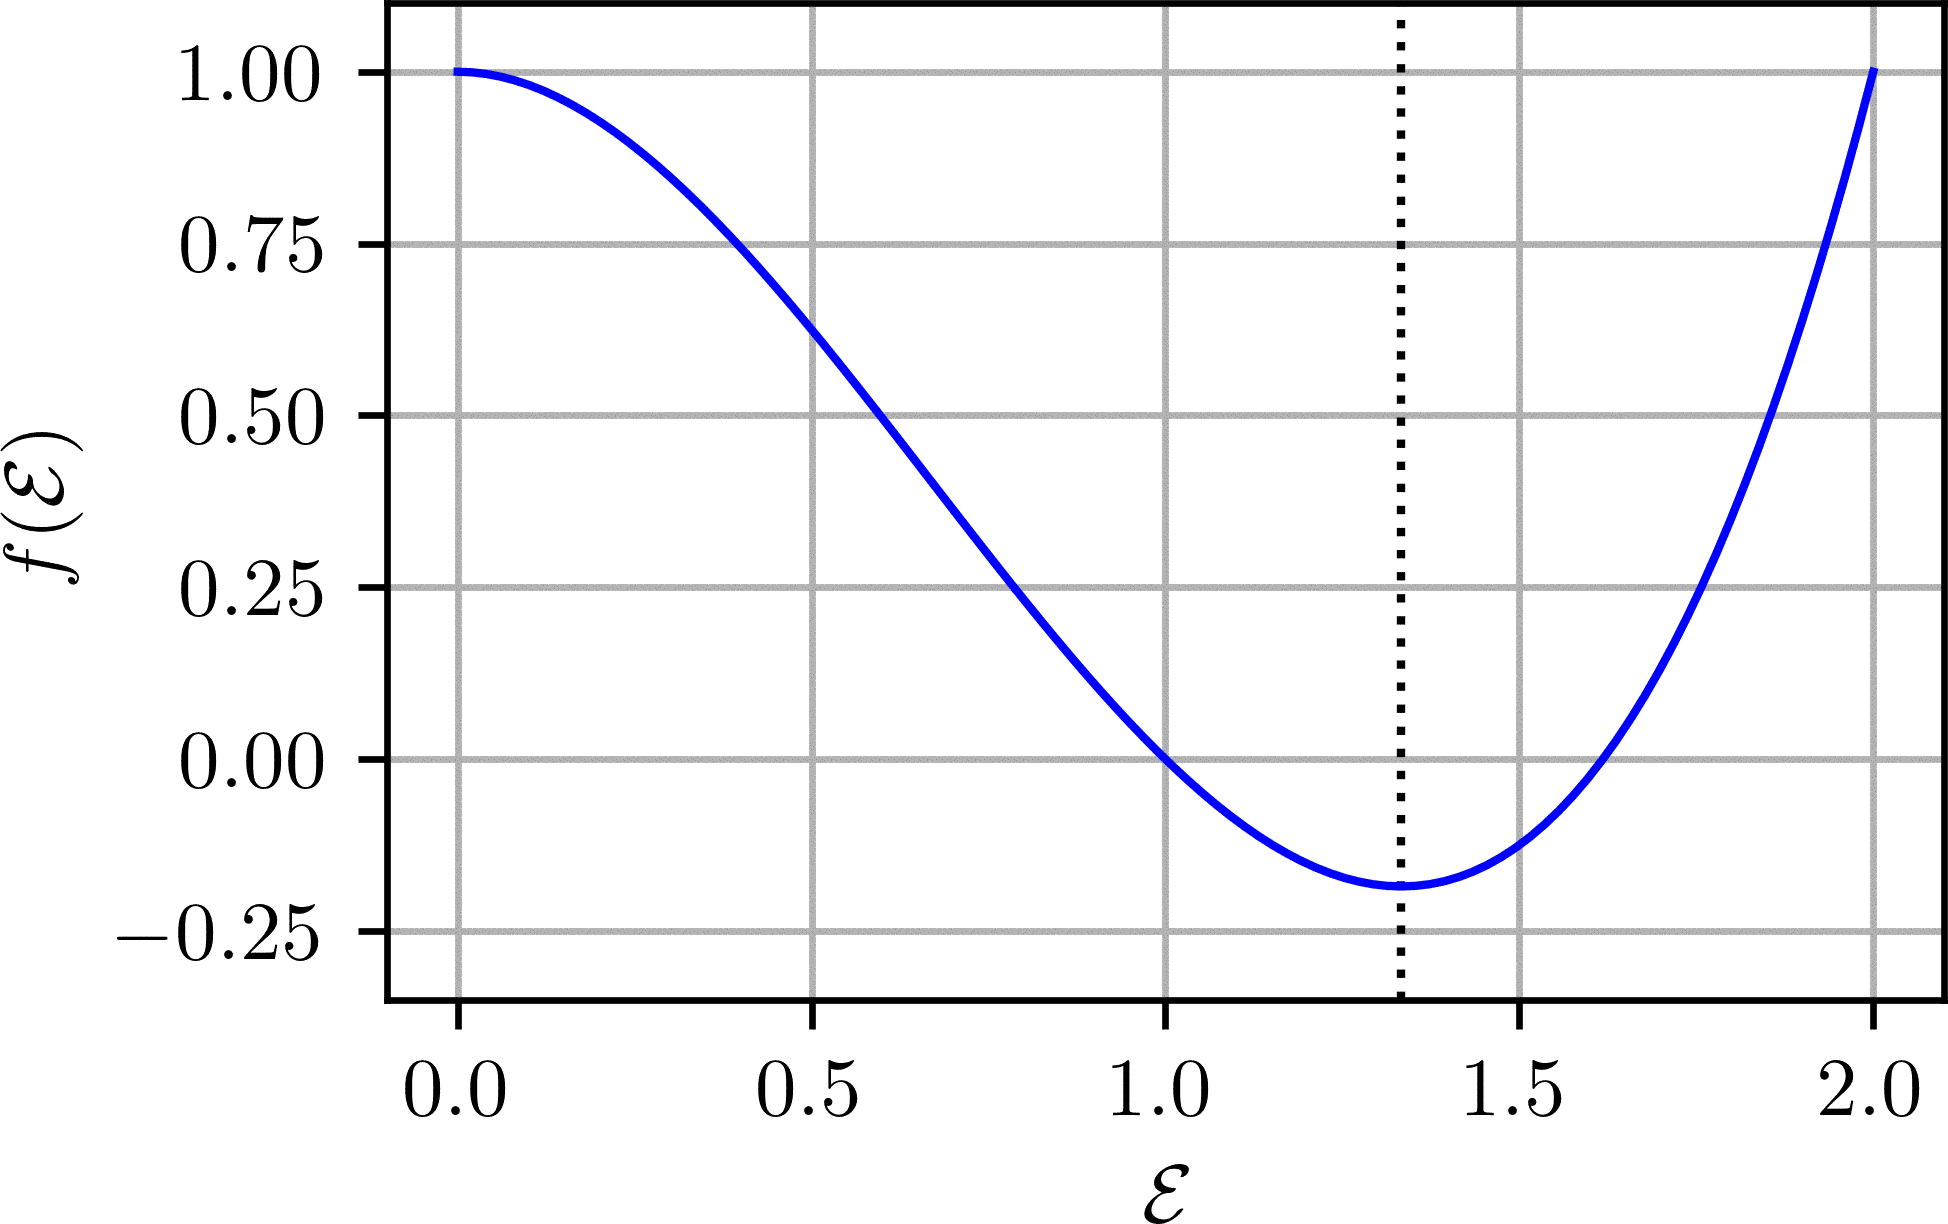
\includegraphics[width=0.5\textwidth]{f_of_Eps.png}
    \caption{Illustration showing that $f(2a/3)\leq0$ in order for
      $f(\Eps)$ to have a positive-valued root. The dashed, vertical
      line corresponds to $\Eps=2a/3$.}
    \label{fig:f_of_Eps}
\end{figure}

Having asserted that $0\leq d \leq (4/27)a^{3}$, we can introduce a variable $\phi\in[0,\pi/2]$ and write, for later convenience,

\eq{
  d = \frac{4}{27}a^{3}\cos^{2}\phi\ .
}

\noindent We claim without proof that the three roots of the polynomial~\eqref{eq:Newmanf} can be written as\footnote{It can be easily checked in a computer algebra software, such as {\tt Mathematica}, that this is indeed true.}

\eq{
  \Eps^{(\ell)} = \frac{a}{3} - \frac{2a}{3}\cos^{2}\left[\frac{2}{3}\left(\phi+\ell\pi\right)\right]\ ,
}

\noindent with the roots corresponding to $\ell=1$, $\ell=2$, and $\ell=3$. The root we are interested in corresponds to $\ell=1$ and we shall provide here the argument given in~\cite{newman2014primitive}. In the limit $\phi\to\pi/2$, it follows that $d\to0$, $\Eps^{(1)}\to a$, $\Eps^{(2)}\to 0$, and $\Eps^{(3)}\to 0$. In this case it is then obvious that $\ell=1$ corresponds to the root we seek. In the limit $\phi\to0$, it follows that $d\to4a^{3}/27$, $\Eps^{(1)}\to2a/3$, $\Eps^{(2)}\to2a/3$, and $\Eps^{(3)}\to -a/3$. The behaviour where the two positive roots converge to the point $\Eps=2a/3$ can be viewed in figure~\ref{fig:f_of_Eps}. We argue then that the branch $\ell=1$ is always the correct one to pick and hence the root $\Eps^{(1)}$ is always the one we are after.

\subsection{The Kastaun \etal scheme}

We now present the recently proposed scheme by Kastaun \etal~\cite{kastaun2021robust}, which is intended to be superior to all the previous one. That being said, as of this writing (Feb. 21, 2021), the scheme has not been tested with fully tabulated equations of state, as far as I am aware. Major advantages of this scheme is that it does not rely on accurate initial guesses and the inversion is guaranteed to succeed, even when the conservative variables are invalid.

We start by defining fluid-only variables

\al{
  D_{\rm fluid} &\equiv D\ ,\\
  \tau_{\rm fluid} &\equiv \tau - b^{2}\left(W^{2} - \frac{1}{2}\right) + \left(\udotB\right)^{2} = D\left(hW - 1\right) - P\ ,\\
  S_{{\rm fluid},i} &\equiv S_{i} - B^{2}\varv_{i} + \frac{\BdotS}{z}B_{i} = DWh\varv_{i}\ .
}

\noindent We now define the order unity auxiliary variables\footnote{Caution: the notation in this section is slightly different than the notation used in previous sections.}

\al{
  \bar{q} \equiv \frac{\tau_{\rm fluid}}{D}\ ,&\quad \bar{r}_{i}\equiv\frac{S_{{\rm fluid},i}}{D}\ ,\\
  q \equiv \frac{\tau}{D}\ ,&\quad r_{i} \equiv \frac{S_{i}}{D}\ ,\\
  \bar{b}_{i} \equiv \frac{B_{i}}{\sqrt{D}}\ ,&\quad \bar{b} \equiv \sqrt{\bar{b}^{i}\bar{b}_{i}}\ .
}

\noindent It is also useful to decompose the momentum part into parts which are normal and parallel to the magnetic field, i.e.

\eq{
  r^{i}_{\parallel} = \frac{\bar{b}^{j}r_{j}}{\bar{b}^{2}}\bar{b}^{i}\ ,\quad r_{\perp}^{i} = r^{i} - r^{i}_{\parallel}\ .
}

\noindent Note that $r^{i}_{\parallel}$ is ill-defined whenever the magnetic field is zero, but below we will only consider the quantity $\bar{b}^{2}r^{i}_{\parallel}$, whiich is always well-defined.

We then define the key variables

\eq{
  \mu \equiv \frac{1}{hW}\ ,\quad x \equiv \frac{1}{1 + \mu \bar{b}^{2}}\ ,
}

\noindent which are limited to

\eq{
  0<\mu\leq\frac{1}{h_{0}}\ ,\quad 0<x\leq1\ ,
}

\noindent where $h_{0}$ is either the minimum enthalpy allowed by the EOS or the value of the enthalpy when $\rho=0$, I am not sure. Starting from the definition of $\bar{r}_{i}$ we have

\spl{
  \bar{r}^{i} &\equiv \frac{\gamma^{ij}S_{{\rm fluid},j}}{D}\\
  &= \frac{1}{D}\left(\gamma^{ij}S_{j} - B^{2}\varv^{i} + \frac{\BdotS}{z}B^{i}\right)\\
  &= \frac{S^{i}}{D} - \frac{B^{2}}{D}\varv^{i} + \frac{\BdotS}{z}\frac{B^{i}}{D}\\
  &= r^{i} - \bar{b}^{2}\left(\frac{S^{i}_{\rm fluid}}{D h W}\right) + \frac{\BdotS}{\rho h W^{2}}r^{i}\\
  &= r^{i} - \mu\bar{b}^{2}\bar{r} + \frac{\mu}{\cancel{D}}\left(\cancel{D}\bar{b}^{j}r_{j}\right)r^{i}\\
  &= - \mu\bar{b}^{2}\bar{r}^{i} + r^{i} + \mu\bar{b}^{2}\left(\frac{\bar{b}^{j}r_{j}}{\bar{b}^{2}}\right)r^{i}\\
  &= - \mu\bar{b}^{2}\bar{r}^{i} + r^{i} + \mu\bar{b}^{2}r^{i}_{\parallel}\\
  &= - \mu\bar{b}^{2}\bar{r}^{i} + r^{i} + \left(\frac{1}{x}-1\right)r^{i}_{\parallel}\\
  &= - \mu\bar{b}^{2}\bar{r}^{i} + r^{i}-r^{i}_{\parallel} + \frac{r^{i}_{\parallel}}{x}\\
  &= - \mu\bar{b}^{2}\bar{r}^{i} + r^{i}_{\perp} + \frac{r^{i}_{\parallel}}{x}\ .
}

\noindent From the last equality we have

\spl{
  \left(1 + \mu\bar{b}^{2}\right)\bar{r}^{i} = \frac{\bar{r}^{i}}{x} = r^{i}_{\perp} + \frac{r^{i}_{\parallel}}{x} \implies \bar{r}^{i} = x r^{i}_{\perp} + r^{i}_{\parallel}\ .
}

\noindent Then we have

\eq{
  \bar{r}^{2} = x^{2}r^{2}_{\perp} + r^{2}_{\parallel}\ ,
}

\noindent since, by construction,

\eq{
  r^{i}_{\perp}r_{\parallel,i} = \left(\frac{\bar{b}^{j}r_{j}}{\bar{b}^{2}}\bar{b}^{i}\right)\left(r_{i} - \frac{\bar{b}^{j}r_{j}}{\bar{b}^{2}}\bar{b}_{i}\right)
  = \frac{\left(\bar{b}\cdot r\right)^{2}}{\bar{b}^{2}} - \frac{\left(\bar{b}\cdot r\right)^{2}}{\bar{b}^{4}}\bar{b}^{2} = 0\ .\label{eq:rbarsq}
}

\noindent Another useful identity is

\spl{
  \bar{q} &\equiv \frac{\tau_{\rm fluid}}{D}\\
  &= \frac{\tau}{D} + \frac{1}{D}\left[- B^{2} - \cancel{\left(\udotB\right)^{2}} + \frac{B^{2} + \left(\udotB\right)^{2}}{2W^{2}} + \cancel{\left(\udotB\right)^{2}}\right]\\
  &= q - \bar{b}^{2} + \frac{\bar{b}^{2}}{2W^{2}} + \frac{\left(\BdotS\right)^{2}}{2z^{2}D}\\
  &= q + \bar{b}^{2}\left(\frac{1}{2W^{2}} - 1\right) + \frac{\mu^{2}}{2}\frac{\left(\BdotS\right)^{2}}{D^{3}}\\
  &= q + \bar{b}^{2}\left(\frac{1}{2W^{2}} - 1\right) + \frac{\mu^{2}}{2}\left(\bar{b}\cdot r\right)^{2}\\
  &= q + \bar{b}^{2}\left(\frac{1}{2W^{2}} - 1\right) + \frac{\mu^{2}}{2}\bar{b}^{2}r^{2}_{\parallel}\\
  &= q + \bar{b}^{2}\left(\frac{1}{2W^{2}} - 1\right) + \frac{1}{2}\mu^{2}\bar{b}^{2}\bar{r}^{2} - \frac{1}{2}\mu^{2}x^{2}\bar{b}^{2}r^{2}_{\perp}\\
  &= q - \frac{\bar{b}^{2}}{2} - \frac{1}{2}\mu^{2}x^{2}\bar{b}^{2}r^{2}_{\perp} + \frac{\bar{b}^{2}}{2}\left[-\left(1 - \frac{1}{W^{2}}\right) + \mu^{2}\bar{r}^{2}\right]\\
  &= q - \frac{\bar{b}^{2}}{2} - \frac{1}{2}\mu^{2}x^{2}\bar{b}^{2}r^{2}_{\perp}\ ,
}

\noindent where in the $6^{\rm th}$  equality we used result~\eqref{eq:rbarsq} and in the last one we used

\eq{
  \mu^{2}\bar{r}^{2} = \mu^{2}\mu^{2}\frac{D^{2}\left(hW\right)^{2}v^{2}}{D^{2}} = \mu^{2}\frac{v^{2}}{\mu^{2}} \implies -\left(1-\frac{1}{W^{2}}\right) + \mu^{2}\bar{r}^{2} = -v^{2} + v^{2} = 0\ .
}

\clearpage
\printbibliography

\end{document}
